\documentclass{article}
\usepackage{neurips_2026}
\usepackage[T1]{fontenc}
\usepackage[utf8]{inputenc}
\usepackage{microtype}
\usepackage{amsmath,amssymb,amsthm,mathtools}
\usepackage{booktabs,tabularx,array}
\usepackage{enumitem}
\usepackage{xcolor}
\usepackage{hyperref}
\usepackage[nameinlink,capitalize]{cleveref}
\usepackage{natbib}
\usepackage{tikz}
\usetikzlibrary{arrows.meta,positioning,fit,shapes.misc}
\newtheorem{definition}{Definition}
\newtheorem{theorem}{Theorem}
\newtheorem{proposition}{Proposition}
\newcommand{\Reach}{\operatorname{Reach}}
\newcommand{\Acc}{\operatorname{Acc}}
\newcommand{\llbracket}{[\![}
\newcommand{\rrbracket}{]\!]}
\definecolor{accent}{RGB}{140,28,38}
\hypersetup{colorlinks=true,linkcolor=accent,citecolor=accent,urlcolor=accent}
\setlist{nosep,leftmargin=*}

\title{Who Repairs After Verification? Evidence-Gated Hierarchies for Local Recovery in Long-Horizon Agents}
\author{Anonymous Authors}
\begin{document}
\maketitle
\begin{abstract}
Verification in long-horizon agents is not only a binary judging problem. A useful verifier must connect evidence to a bounded claim, localize what became stale, and decide whether to accept, repair locally, replan upward, or request human authority. We present an evidence-gated hierarchy in which an approved Plan is refined into Phases, durable intent contracts (DICs), disposable execution plans, and evidence-linked actions. Under complete dependency declarations and version-bound evidence, we prove that repair can safely retain artifacts outside the dynamic impact cone and that this cone is worst-case tight. If each gate's conditional miss probability is at most $\alpha$, fault survival falls as $\alpha^k$; conversely, evidence aliasing makes simultaneous zero false acceptance and rejection impossible. The package implements these semantics and a deterministic locality smoke test, but has no confirmatory language-agent comparison. We therefore define a matched-budget fault-injection protocol measuring unsupported completion, detection latency, propagation, and rework against flat and verifier-only controls.
\end{abstract}

\section{Verification must choose a recovery scope}
Agent verification is often represented as a score or critique appended to generation. On a long dependency chain, that leaves three unresolved questions: what exact claim was checked, which downstream artifacts relied on it, and whether failure should trigger a local retry or invalidate the plan. A late binary ``incorrect'' can be almost as costly as no verifier when it causes a full rerun; a confident ``correct'' can be dangerous when the evidence did not observe the relevant property.

We treat verification as a closed-loop state transition rather than an extra response. The durable hierarchy is
\[
\text{Plan}\to\text{Phase}\to\text{DIC}\to\text{EPS}\to\text{Prompt/Run}\to\text{Action}\to\text{evidence}.
\]
The DIC binds a bounded subgoal to constraints, authority, acceptable-state predicates, evidence requirements, dependencies, and escalation triggers. Verification returns $\mathsf{accept}$, $\mathsf{repair}$, $\mathsf{replan}$, or $\mathsf{escalate}$. Repair regenerates operations under the same contract; replan changes its semantic parent; escalation stops autonomy for a material decision.

This paper contributes the verification/recovery semantics, formal locality and observability results, a package-resident implementation, and an experiment that separates verifier inference from verifier-guided local repair. Hierarchical planning itself and verifier calls are not claimed as new \citep{yao2023react,shinn2023reflexion,lightman2023verify}.

\section{Evidence-gated hierarchy}
A Plan is a human-approved DAG spanning several machine phases. Human review is periodic rather than per phase, with immediate escalation for scientific, protocol, release, destructive/external, paid-compute, or credential changes. Main, Theory, and Experiment own distinct scientific workstreams. Every Action record points to an EPS, DIC, Phase, and Plan; the package, not chat history, stores authority.

For a phase ending at state $s$ with evidence $e$, acceptance is
\[
\Acc_C(s,e)=\mathbf 1\{s\in A_C,\ I_C\text{ held},\ W_C(s,e)=1\}.
\]
$A_C$ states what is acceptable; $W_C$ states what evidence warrants that assertion. This separation prevents a test log from silently becoming evidence for a broader scientific claim.

\begin{figure}[t]
\centering
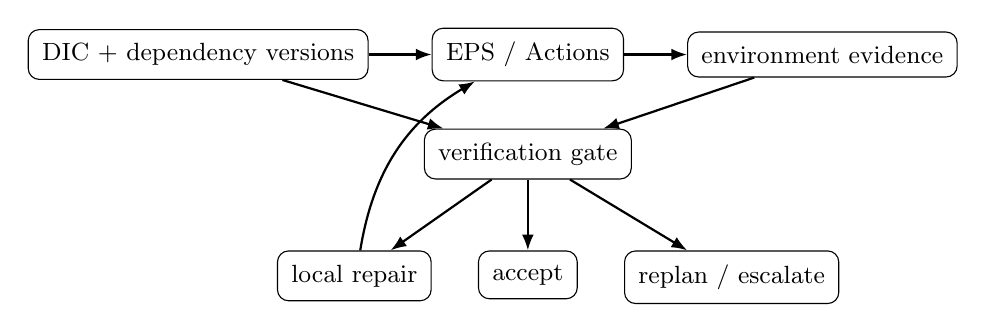
\begin{tikzpicture}[node distance=6mm and 8mm, every node/.style={font=\small}, box/.style={draw,rounded corners,inner sep=5pt}, arr/.style={-{Latex[length=2mm]},thick}]
\node[box] (dic) {DIC + dependency versions};
\node[box,right=of dic] (exec) {EPS / Actions};
\node[box,right=of exec] (ev) {environment evidence};
\node[box,below=of exec] (ver) {verification gate};
\draw[arr] (dic)--(exec);\draw[arr] (exec)--(ev);\draw[arr] (ev)--(ver);\draw[arr] (dic)--(ver);
\node[box,below left=9mm and -1mm of ver] (rep) {local repair};
\node[box,below=9mm of ver] (acc) {accept};
\node[box,below right=9mm and -1mm of ver] (up) {replan / escalate};
\draw[arr] (ver)--(rep);\draw[arr] (ver)--(acc);\draw[arr] (ver)--(up);\draw[arr,bend left=25] (rep) to (exec);
\end{tikzpicture}
\caption{Verification is coupled to evidence, dependency versions, and recovery scope.}
\label{fig:loop}
\end{figure}

\section{Local recovery and its limit}
Let state be keyed by $\mathcal K$. Phase $v$ declares reads $R_v$ and writes $W_v$; every possible data dependence is an edge. A repair changes keys $\Delta$. Define the direct readers $B(\Delta)=\{v:R_v\cap\Delta\ne\varnothing\}$ and impact cone $\mathcal I(\Delta)=\Reach(B(\Delta))$.

\begin{theorem}[Safe local invalidation]
Assume complete read/write declarations, no hidden mutable state, evidence bound to input/artifact versions, and phase semantics determined by declared inputs and recorded tool/randomness parameters. Then completed outputs outside $\mathcal I(\Delta)$ remain contract-valid after the repair.
\end{theorem}
\begin{proof}[Sketch]
A node outside the cone neither reads $\Delta$ nor depends on a changed predecessor. Topological induction preserves its declared inputs, outputs, and version-bound evidence.
\end{proof}
The cone is worst-case necessary. A direct reader can copy one changed bit; phases along any path can propagate it, making every descendant's previous evidence stale. The theorem is therefore only as trustworthy as the dependency declarations. It adapts incremental-build locality to agent artifacts \citep{mokhov2018build,acar2009selfadjusting}.

\section{Imperfect and insufficient verifiers}
Suppose a persisting observable fault is missed at each gate with conditional probability at most $\alpha<1$. By the chain rule, survival through $k$ gates is at most $\alpha^k$, and expected detection delay is at most $1/(1-\alpha)$ gate intervals. This does not require independent errors, but it does require the conditional bound to remain valid.

More fundamentally, let evidence observation be $O(s)$. If $O(s_+)=O(s_-)$ while the goal holds only in $s_+$, any evidence-only verifier makes the same decision on both and therefore incurs a false acceptance or false rejection. Verification quality cannot exceed the information in its environment-grounded evidence. Additional critique tokens do not resolve an unobserved distinction.

A stylized checkpoint model further shows that review cadence depends on cost and verifier quality. With checkpoint/false-rejection cost $c_v+\beta c_f$, fault rate $\lambda$, repair cost $c_r$, and miss rate $\alpha$, the continuous optimum is
\[
h^*=\sqrt{\frac{2(c_v+\beta c_f)(1-\alpha)}{\lambda c_r(1+\alpha)}}.
\]
This is an operating trade-off, not a universal recommendation \citep{young1974first,daly2006higher}.

\section{Implementation and current evidence}
The standard-library runtime stores a canonical index plus multi-view DIC, EPS, prompt/run, and Action records. It implements Plan approval, autonomous ordinary progression, dependency blocking, periodic checkpoints, immediate material escalation, four verification outcomes, hash-checked lineage, package-only recovery, and v5.6.31 migration aliases. The release package records exact test and recovery logs.

A deterministic seven-node fixture changes one key. Four nodes lie in the declared impact cone, so three unaffected nodes are retained. This validates the implementation of the formal invalidation rule under known dependencies. It is not evidence that an LLM will declare dependencies correctly or outperform a flat agent.

\section{Fault-injection evaluation}
We freeze four main conditions: C0 direct/reactive; C1 flat plan-and-execute; C2 hierarchy without gated recovery; C3 hierarchy with verification-triggered repair/replanning. C1+V uses the same verifier-call budget for generic critique but lacks dependency-local repair; C2-extra spends the budget on additional generation. All conditions share the base model, tool access, task information, and matched token/call budget or are compared on a Pareto frontier.

Tasks vary dependency depth, branching, delayed dependencies, interacting constraints, and hidden faults (stale schemas, omitted constraints, version swaps, corrupted statistics, unsupported citations, failing code). Objective graders measure end-to-end success and constraint satisfaction. Verification-specific primary outcomes are unsupported completion, false-acceptance proxies, detection latency, downstream propagation, recovery locality, and rework. The central test is whether C3's advantage over C1/C2 grows with effective horizon and exceeds verifier-only controls.

No comparative numbers appear until prompts, graders, seeds, budgets, stopping rules, and exclusions are frozen and at least two task families complete. Unit tests and fixtures remain smoke evidence.

\section{Relation to verification and oversight}
Reflexion and search-based agents use feedback to improve subsequent actions \citep{shinn2023reflexion,zhou2024lats}. Process supervision and scalable oversight study how weaker or intermediate signals can guide stronger systems \citep{lightman2023verify,irving2018debate,leike2018recursive,burns2024weakstrong}. ToolEmu and AgentDojo emphasize environment and adversarial risks \citep{ruan2024toolemu,debenedetti2024agentdojo}. Our narrower focus is the contract/evidence object and invalidation semantics that turn a verification outcome into a bounded recovery decision across persistent artifacts.

\section{Limitations and conclusion}
Hidden dependencies, weak acceptance predicates, correlated verifier errors, mutable services, and adversarial evidence can all defeat the mechanism. The runtime does not create a semantic oracle or security boundary. Human checkpoints may still be too sparse for high-impact domains, and role separation is not independence. The current package establishes a testable verification architecture, formal conditions, and engineering conformance---not end-to-end superiority. Its central proposition for future evidence is operational: a verifier is most useful when it can say not only \emph{whether} an artifact failed, but \emph{what evidence failed, what must be invalidated, and at what authority level execution should resume}.

\bibliographystyle{plainnat}
\bibliography{references}
\end{document}
